\section{Intranet des maisons d'édition Eyrolles}

\subsection{Contexte et objectifs}

TODO

\subsubsection{Planning initial}

TODO

\subsection{Organisation du travail}

\subsubsection{Phase d'analyse}

TODO

\subsubsection{Phase de développement}

TODO

\subsubsection{Phase de recette}

TODO

\subsubsection{Livraison finale}

TODO

\subsubsection{Planning réel}

TODO

\subsection{Fonctionnalités attendues de l'Intranet}

TODO

\subsection{\textit{slAdminPlugin}}

La plupart des vues du lot~2 de l'Intranet d'Eyrolles sont générées grâce au plugin Symfony \textit{slAdminPlugin}. Il a été développé en interne par Sensio Labs et est issu de l'abstraction du code d'un précédent projet. Il n'a rien à voir avec la fonctionnalité de génération d'administration intégrée à Symfony. C'est encore un plugin très jeune : Eyrolles est le premier projet qui l'utilise.

\begin{table}
	\centering
	\begin{tabular}{|p{3cm}||p{4.5cm}|p{4.5cm}|}
		\hline
		& Génération d'administration & \textit{slAdminPlugin} \tabularnewline
		\hline
		\hline
		Format de configuration & YAML & code PHP \tabularnewline
		\hline
		Génération de code & oui & non \tabularnewline
		\hline
		Personnalisation de la logique & surcharge de code généré & surcharge de méthodes d'action de base \tabularnewline
		\hline
		Personnalisation des vues & surcharge de \textit{partials} générés & écriture classique de \textit{templates} \tabularnewline
		\hline
	\end{tabular}
	\caption{Comparaison entre la génération d'administration de Symfony et \textit{slAdminPlugin}}
	\label{table:eyrolles_sladmin-vs-admin-gen}
\end{table}

Le tableau~\ref{table:eyrolles_sladmin-vs-admin-gen} reprend une comparaison rapide des différences entre le moteur de génération d'administration de Symfony et \textit{slAdminPlugin}. Le plugin, tout comme la génération d'administration, permet de ne pas avoir à redévelopper la logique des opérations de base, telles que le listing d'éléments, la pagination et le tri de la liste, ou encore la création, l'édition ou la suppression d'éléments. Sa valeur ajoutée est qu'il apporte plus de flexibilité quant à la personnalisation de la logique et des différentes vues.

Un exemple d'implémentation de module utilisant \textit{slAdminPlugin} sera présenté dans la partie~\ref{section:eyrolles_ref-langues}

\textit{slAdminPlugin} s'articule autour de trois composants majeurs :
\begin{itemize}
	\item une classe PHP de configuration ;
	\item des actions d'administration de base ;
	\item des widgets pour agencer la vue.
\end{itemize}

\subsubsection{La classe de configuration}

La classe de configuration permet de stocker les différents paramètres qui seront utilisés pour configurer les actions et la vue d'un module.

Une classe de configuration doit satisfaire les conditions suivantes :
\begin{itemize}
\item elle doit être placée dans le dossier \texttt{lib/config} du module et doit être nommée \texttt{slAdminConfigurationMonNomDeModule};
\item elle doit hériter de la classe abstraite \texttt{slBaseAdminConfiguration} du plugin, qui contient la liste de toutes les options disponibles (cf. Figure~\ref{figure:eyrolles_sladmin-config}) ;
\item la définition des paramètres personnalisés doit se faire dans la méthode \texttt{configure()} surchargée.
\end{itemize}

\begin{figure}
	\centering
	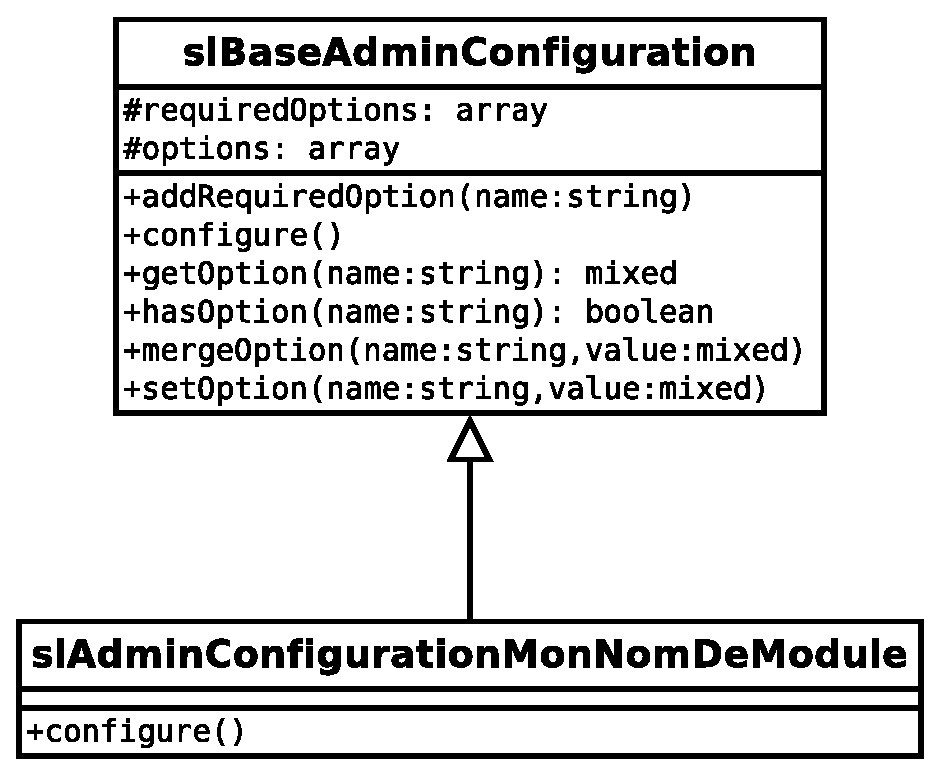
\includegraphics[scale=0.4]{eyrolles_sladmin-config}
	\caption{Classe de configuration de \textit{slAdminPlugin}}
	\label{figure:eyrolles_sladmin-config}
\end{figure}

\subsubsection{Actions de base}

\textit{slAdminPlugin} contient deux classes d'actions qui servent de base aux actions des modules gérés.

La première, \texttt{slBaseActions}, hérite de la classe Symfony \texttt{sfActions}. Elle fournit des méthodes pour gérer les messages de confirmation ou les messages d'erreur, ainsi qu'une méthode de validation de formulaire avancée. La seconde classe, \texttt{slAdminActions}, hérite de \texttt{slBaseActions}. C'est elle qui contient toutes les actions d'administration supportées telles que \texttt{show}, \texttt{list}, \texttt{edit}, \texttt{delete}, \texttt{filter}, \texttt{sort} ou \texttt{batch}.

Ainsi, la classe d'actions d'un module utilisant \textit{slAdminPlugin} doit hériter de la classe \texttt{slAdminActions} au lieu de la classique \texttt{sfActions}. Les méthodes d'action peuvent alors être surchargées si nécessaire.

Ce comportement est décrit dans la Figure~\ref{figure:eyrolles_sladmin-actions}.

\begin{figure}
	\centering
	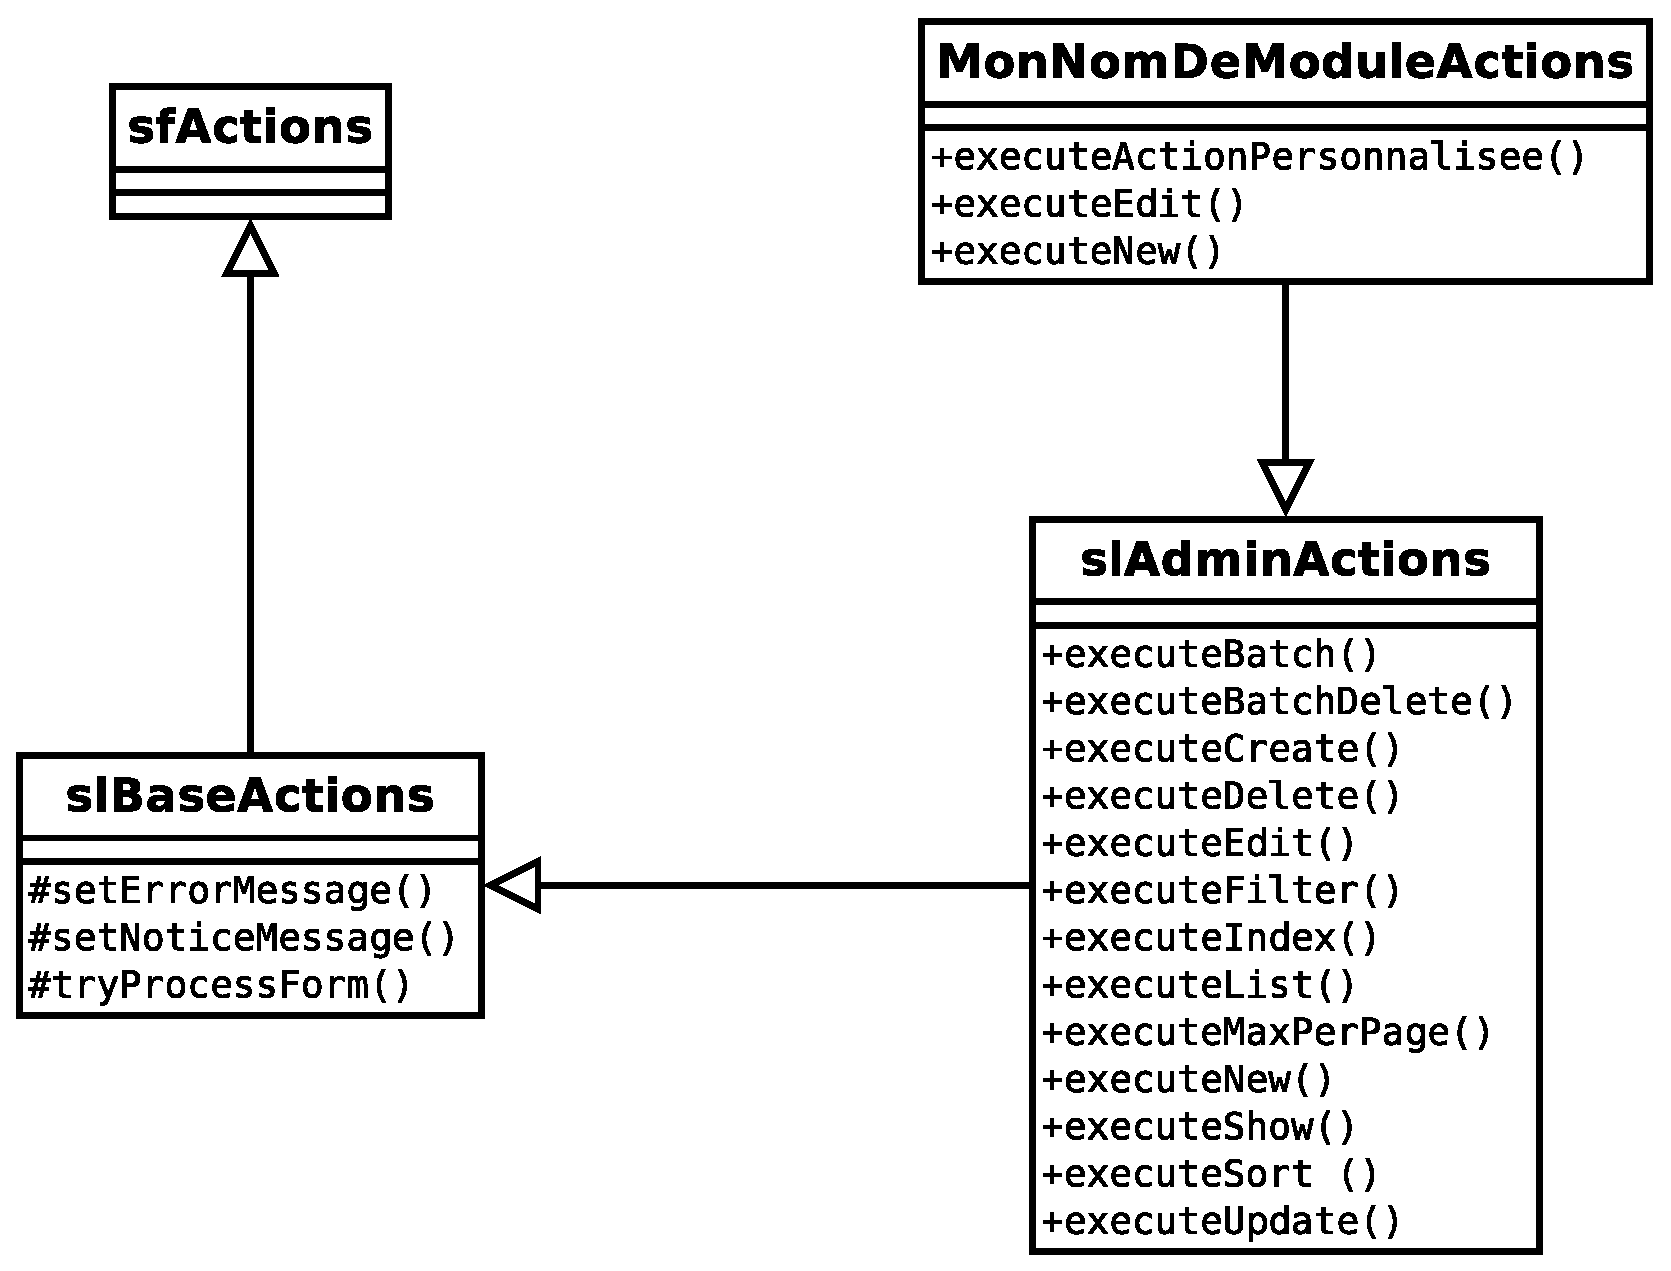
\includegraphics[scale=0.4]{eyrolles_sladmin-actions}
	\caption{Actions de base fournies par \textit{slAdminPlugin}}
	\label{figure:eyrolles_sladmin-actions}
\end{figure}

\subsubsection{Gestion de la vue}

À la base, un module utilisant \textit{slAdminPlugin} doit posséder les cinq \textit{templates} suivants :
\begin{description}
	\item[\texttt{listSuccess.php}] -- le \textit{template} affichant le listing des objets du modèle géré par le module, contenant par exemple les filtres, un tableau d'affichage et un pager ;
	\item[\texttt{listHeader.php}] -- le \textit{partial} affichant la ligne de titre du tableau de listing ;
	\item[\texttt{list\_row.php}] -- le \textit{partial} affichant une ligne du tableau de listing ;
	\item[\texttt{newSuccess.php}] -- le \textit{template} affichant le formulaire de création d'objet ;
	\item[\texttt{editSuccess.php}] -- le \textit{template} affichant le formulaire d'édition d'objet.
\end{description}

Les éléments récurrents de ces vues comme le tableau d'affichage des objets ou le pager sont en réalité des \textit{widgets}, qui sont instanciés dans les actions de base de \textit{slAdminPlugin}. Le nom des classes de ces \textit{widgets} peuvent d'ailleurs être définis dans la classe de configuration du module. Les \textit{widgets} peuvent être affichés dans un \textit{template} comme le montre le Listing~\ref{listing:eyrolles_sladmin-template}.

\lstinputlisting[float, caption={Affichage de \textit{widgets} de \textit{slAdminPlugin} dans un \textit{template}}, label={listing:eyrolles_sladmin-template}]{code/eyrolles_sladmin-template.php}


\subsection{Un module type : le référentiel des langues}
\label{section:eyrolles_ref-langues}

Le référentiel des langues est l'un des nombreux référentiels administrables de l'application décrits dans la partie~***.

Il est implémenté sous la forme d'un module nommé \texttt{ey\-Referential\-Language} qui utilise \asladmin. En effet, le module doit offrir les fonctionnalités suivantes, qui sont offertes par défaut par le \aplugin\ :
\begin{itemize}
\item le listings des langues contenues dans la base de données ;
\item l'ajout et la modification d'une langue ;
\item la suppression d'une langue.
\end{itemize}

Le module des langues a été choisi pour être décrit car il peut être considéré comme un module qui, tout en restant très simple, est typique de l'application. Les paragraphes suivants rentrent dans le détail de son implémentation, et l'annexe~\ref{section:annexe_eyrolles_ref-langues} regroupe son code et des captures d'écran.


\subsubsection{Arborescence}

L'arborescence de \texttt{eyReferentialLanguage} suit les règles classiques d'organisation d'un module \asf\ et intègre les fichiers nécessaires au bon fonctionnement de \asladmin\ :

\begin{verbatim}
eyReferentialLanguage/
  actions/
    actions.class.php
  lib/
    config/
      slAdminConfigurationEyReferentialLanguage.class
  templates/
    _form.php
    _listTableRow.php
    listSuccess.php
    newSuccess.php
\end{verbatim}

L'organisation des fichiers de \atemplate\ ne suit pas exactement les consignes énoncées en partie~\ref{section:eyrolles_sladmin_view}. En effet, dans la classe de configuration, on a préféré utiliser le nom de \apartial\ \texttt{listTableRow} au lieu de \texttt{list\_row}. Par ailleurs, le \apartial\ \texttt{form} est appelé dans le \atemplate\ \texttt{new}.


\subsubsection{Schéma de la base de données}

Le données du référentiel des langues sont stockées dans une seule table de la base de données nommée \texttt{EyReferentialLanguage}. Elle contient les champs suivants : \texttt{id}, \texttt{label}, \texttt{description} et \texttt{created\_by}. Le champ \texttt{id} est la clé primaire de la table, qui sert à identifier de façon unique chaque langue. Quant au champ \texttt{created\_by}, il est utilisé en tant que clé étrangère vers la table des utilisateurs de l'\aintranet\ \texttt{sfGuardUser} : cette liaison permet de retrouver le créateur de la langue.

Le schéma permettant de créer cette table dans la base de données est repris dans le listing~\ref{listing:eyrolles_ref-langues_schema}. Pour expliciter ce format, un diagramme \auml\ équivalent est proposé en figure~\ref{figure:eyrolles_ref-langues_uml}.

\begin{figure}
	\centering
	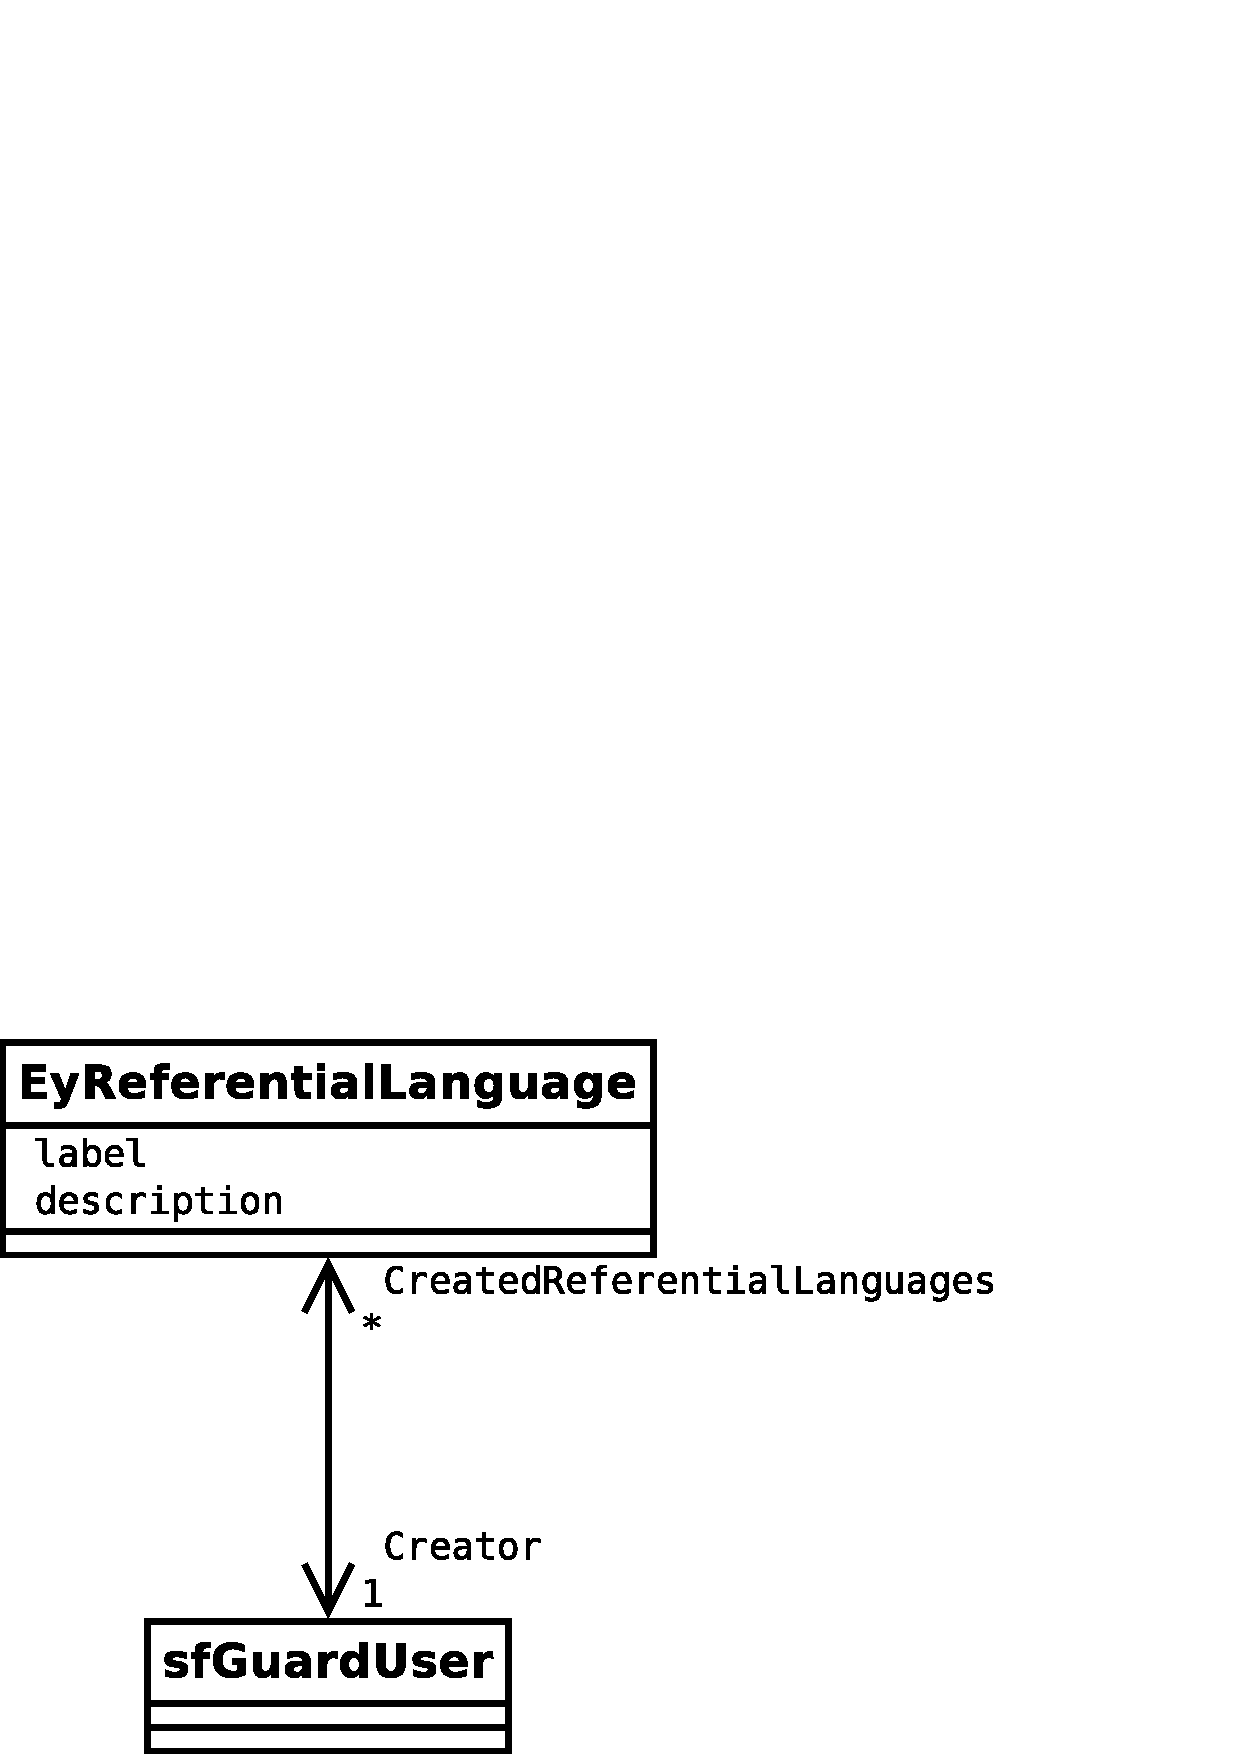
\includegraphics[scale=0.4]{eyrolles_ref-langues_uml}
	\caption{Représentaion \auml\ de la table du référentiel des langues}
	\label{figure:eyrolles_ref-langues_uml}
\end{figure}

On peut noter l'utilisation des mots-clés \texttt{Timestampable} et \texttt{SoftDelete} listés dans la partie \texttt{actAs}. Ce sont ce que l'on appelle des \emph{behaviors} \adoctrine\ : ils peuvent être assimilés à des comportements personnalisés que l'on veut donner à une table.

En effet, le \abehavior\ \texttt{Timestampable} ajoute automatiquement deux champs \texttt{created\_at} et \texttt{updated\_at} dans la table. Respectivement, ils sont remplis automatiquement par une date quand un enregistrement est crée et quand il est mis à jour. En plus de garder une trace du créateur de la langue, \texttt{Timestampable} conservera alors les données temporelles de modification de la table.

Le \abehavior\ \texttt{SoftDelete}, quant à lui, permet de ne jamais supprimer un enregistrement de la base de données. En fait, il ajoute un champ \texttt{deleted\_at} : quand on demande la suppression d'un enregistrement, sa valeur est affectée à la date de la pseudo délétion, sinon sa valeur est nulle. Les différentes requêtes \adoctrine\ écrites par le développeur sont alors automatiquement modifiées pour ignorer les enregistrements qui sont sensés avoir été supprimés. Dans le cas d'\aey, \texttt{SoftDelete} permet d'implémenter nativement l'archivage des données au cas où le client aurait besoin de les restaurer ou d'en générer des statistiques.


\subsubsection{Configuration}

La classe de configuration nécessaire pour \asladmin\ est accessible dans le listing~\ref{listing:eyrolles_ref-langues_config}.

Sans expliciter de façon fastidieuse toutes les options utilisées, elle définit globalement les paramètres suivants :

\begin{itemize}
\item la classe de modèle à utiliser ;
\item la requête à utiliser pour récupérer les langues à afficher sur la page de listing (listing~\ref{listing:eyrolles_ref-langues_table}) ;
\item le champ sur lequel les langues seront triés ;
\item le nombre maximum de langues affichées sur la page de listing ;
\item le titre des colonnes du tableau de la page de listing ;
\item le \apartial\ à utiliser pour afficher une ligne du tableau de listing ;
\item les classes de formulaire à utiliser.
\end{itemize}


\subsubsection{Routes}

Le fichier de \arouting\ du module est accessible dans le listing~\ref{listing:eyrolles_ref-langues_routing}.

\texttt{eyReferentialLanguage\_batch} est une route classique. La valeur du champ \texttt{url} correspond à l'adresse que l'utilisateur va entrer dans son navigateur pour accéder à l'action \texttt{batch} du module \texttt{eyReferentialLanguage}. L'option \texttt{sf\_method} indique quelle méthode HTTP\footnote{Dans le protocole HTTP, une méthode est une commande spécifiant un type de requête, c'est-à-dire qu'elle demande au serveur d'effectuer une action. \cite{http}} l'utilisateur doit appeler pour que la route soit accessible. Dans le cas de cette route, la méthode est \texttt{POST}, ce qui correspond en fait à la validation d'un formulaire.

La route \texttt{eyReferentialLanguage}, quant à elle, utilise la classe de \arouting\ avancée \texttt{sfDoctrineRouteCollection}. Cette classe intégrée au \afm\ \asf\ a la particularité de générer tout un ensemble routes qui correspondent à des actions de bases. Par exemple, des actions générées sont \texttt{ey\-Re\-fe\-ren\-tial\-Lan\-guage\_\-list}, \texttt{ey\-Re\-fe\-ren\-tial\-Lan\-guage\_\-new}, \texttt{ey\-Re\-fe\-ren\-tial\-Lan\-guage\_\-edit}, correspondent respectivement aux actions \texttt{list}, \texttt{new}, \texttt{edit}, et redirigent respectivement vers le listing des langues, la création d'une langue et son édition.


\subsubsection{Actions}

Les actions du module, situées dans la classe \texttt{ey\-Referential\-Language\-Actions}, reposent sur les actions de base d'\aey\footnote{Voir le listing~\ref{listing:eyrolles_base_actions}}, qui reposent elles-mêmes sur les actions de \asladmin. Elles sont accessibles dans le listing~\ref{listing:eyrolles_ref-langues_actions}.

On remarque que seule l'action \texttt{edit} est redéfinie. En effet, on y ajoute le nom de la langue que l'on est en train d'éditer dans le fil d'Arianne\footnote{Sur un site web, un fil d'Ariane représente l'arborescence des rubriques que le visiteur a traversées depuis la page d'accueil.\cite{breadcrumb}\\Exemple : \texttt{Accueil > Référentiels > Langues > Liste}}. Toutes les autres actions comme \texttt{list} ou \texttt{new} sont en réalité déjà écrites dans les actions de base de \asladmin. Le fait qu'il y ait au final peu de code à écrire est un bon signe : c'est un gain de temps pour le développeur et c'est une bonne opportunité pour ne pas intégrer de \abug. C'est justement ce genre d'avantage qui a incité à utiliser \asladmin\ dans \aey.

Dans les actions de base \texttt{eyBaseAdminActions}, la méthode \texttt{init\-Bread\-crumb()}, qui initialise le fil d'Arianne, est appelée dans la méthode \texttt{pre\-Execute()} : ainsi, le fil d'Arianne est initialisé dans chaque action de l'application \aey. La méthode \texttt{initBreadcrumb()} est surchargée dans \texttt{ey\-Referential\-Language\-Actions} : au mot \textit{Accueil} présent sur toute les pages, on ajoute \textit{Référentiels} puis \textit{Langues}. C'est un bon exemple de la façon typique de surcharger les classes de \asladmin.

Le module du référentiel des langues restant un module très simple, les actions de \asladmin\ n'ont pas trop eu a être surchargées. Dans d'autres modules, qui intègrent une logique métier plus poussée, il est nécessaire d'apporter une surcharge plus importante et d'écrire des actions supplémentaires spécifiques.


\subsubsection{Affichage de la vue}

Les vues, contrairement aux actions, n'ont pas déjà été écrites dans \asladmin.


\subsubsection{Formulaire de création-édition}

TODO


\subsection{Utilisation de l'héritage avec Doctrine}

TODO

\subsection{Gestion de la session utilisateur avec \textit{sfGuardDoctrinePlugin}}

TODO

\subsection{Export de données au format CSV}

TODO

\subsection{Webservices}

\subsubsection{Le webservice des auteurs}

TODO

\subsubsection{Refactoring des webservices}

TODO

\subsection{Tâches}

\subsubsection{Tâche d'initialisation des auteurs}

TODO

\subsubsection{Refactoring des tâches}

TODO

\subsection{Écriture de tests}

\subsubsection{Tests unitaires}

TODO

\subsubsection{Tests fonctionnels}

TODO

\subsection{Processus de mise en production}

TODO

\subsection{Bilan}
